\subsection{Message Authentication Codes}\label{sec:symmetric_cryptography:mac}

A \textbf{\gls{mac}} --- also known as a \textit{cryptographic checksum} or \textit{authentication tag} or simply \textit{tag} --- is a sequence of bytes created through a dedicated algorithm taking as input some data and a symmetric key (\Cref{figure:mac_creation_and_verification}). The objective of a \gls{mac} is to detect both accidental and intentional modifications of data \cite{barker_recommendation_2020_p1}. Hence, a \gls{mac} provides integrity and --- if the symmetric key is known by a specific set of two or more parties --- also message authenticity (\Cref{sec:security_properties}). Differently from digital signatures (\Cref{sec:digital_signatures}), \glspl{mac} are verified using the same symmetric key employed to generate them. By themselves, \glspl{mac} do not perform encryption; hence, \glspl{mac} must be combined with (symmetric) encryption to provide confidentiality. There are two main approaches for creating \glspl{mac}: hash-based (\Cref{sec:symmetric_cryptography:hmac}) and block cipher-based (\Cref{sec:symmetric_cryptography:cbc_mac}).

\begin{figure}[t!]
	\begin{center}
		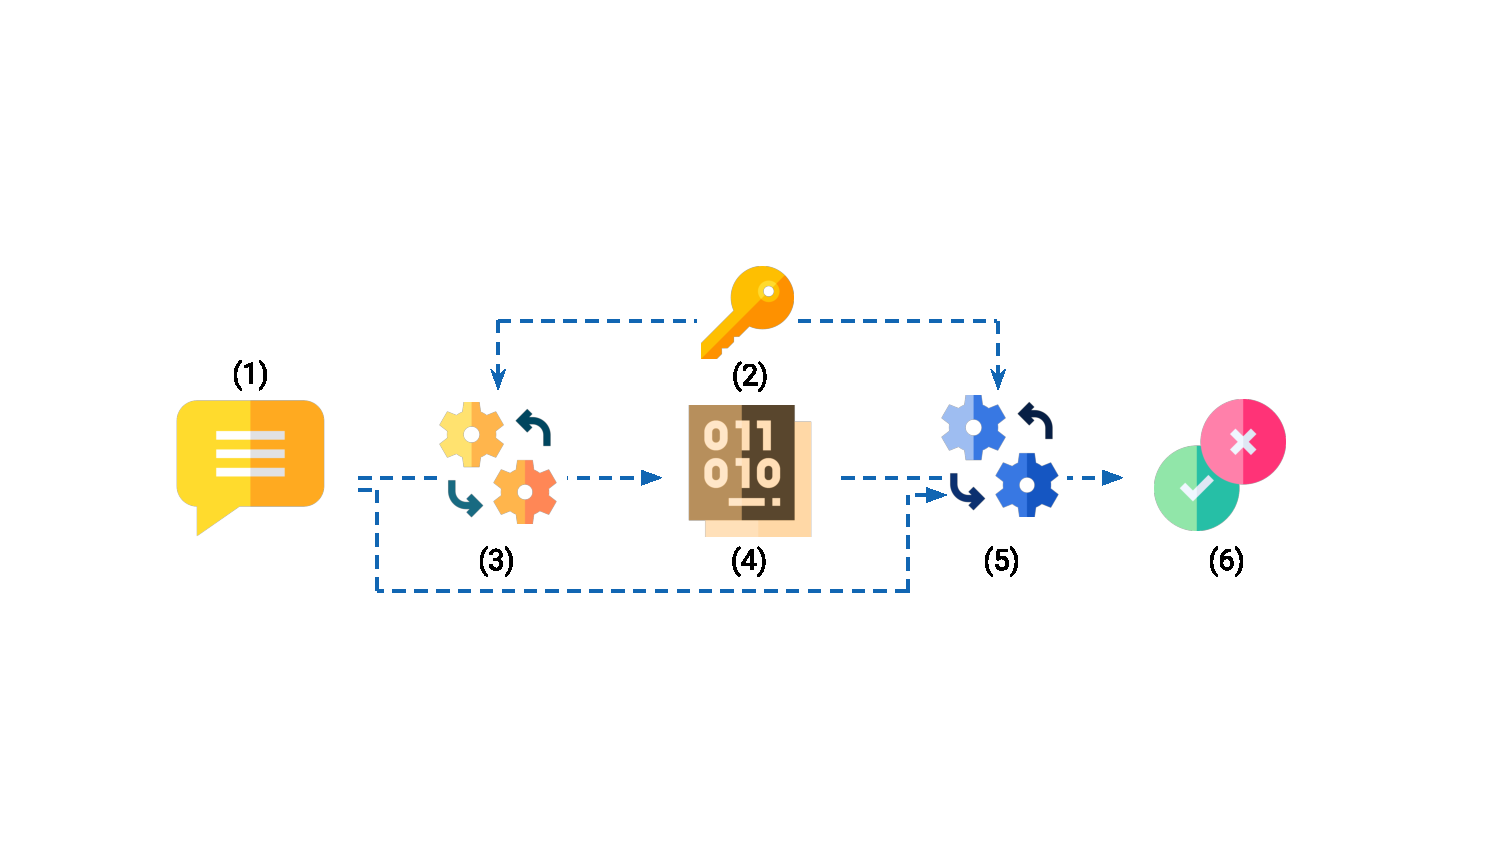
\includegraphics[trim={3cm 4cm 3.5cm 4.5cm},clip,width=0.75\linewidth]{resources/pdf/mac_creation_and_verification.pdf}
		\caption{The process of creating and verifying \glspl{mac}. The data over which the \gls{mac} is created (1) --- any sequence of bytes of arbitrary length --- and a symmetric key (2) are given as input to the \gls{mac} creation algorithm (3) which returns as output the \gls{mac} (4). The \gls{mac} verification algorithm (5) --- which is usually very similar to the \gls{mac} creation algorithm (3) --- takes as input the data (1), the \gls{mac} (4), and the symmetric key (2), and returns as outcome a boolean value (6) --- either the \gls{mac} is valid or it is not.}
		\label{figure:mac_creation_and_verification}
	\end{center}
\end{figure}

\subsubsection{Hash-based Message Authentication Codes}\label{sec:symmetric_cryptography:hmac}

A \textbf{\gls{hmac}} --- also called \textit{keyed-hash \gls{mac}} --- is a \gls{mac} created by wrapping a \gls{chf} (\Cref{sec:hash_functions:cryptographic_hash_function:keyed}) into two keyed hashing operations over combination of a symmetric key and a given message \cite{krawczyk_hmac_1997}. \glspl{hmac} often derive two keys --- inner and outer --- from the symmetric key, and expect two hash computations to resist length extension attacks (\Cref{sec:hash_functions:cryptographic_hash_function:keyed}). \glspl{hmac} are a specific instance of keyed \gls{chf}.

\subsubsection{Cipher Block Chaining Message Authentication Codes}\label{sec:symmetric_cryptography:cbc_mac}

A \textbf{\gls{cbc}-\gls{mac}} --- also called \textit{\gls{cmac}} --- is a \gls{mac} created by applying a block cipher (\Cref{sec:cryptography_basics:ciphers}) to a given message. Usually, the message is encrypted using a block cipher in \gls{cbc} mode with zero \gls{iv}; the last block is the \gls{mac}. \glspl{cmac} are often used in systems where block ciphers are already being used.
